\section{Protocolli di coerenza}
La coerenza può essere definita formalmente tramite un appropriato invariante, scelto equivalentemente tra:

\begin{itemize}
    \item \textbf{SWMR} (Single Writer Multiple Reader): Durante una data epoca, o c'è un singolo core che può leggere o scrivere la locazione A, oppure un numero di cores che possono solo leggerla.
    \item \textbf{DV} (Data Value): Il valore di A all'inizio di un'epoca è lo stesso valore di A alla fine della sua ultima epoca di lettura/scrittura. 
\end{itemize}

\noindent
Altre opzioni per i protocolli di coerenza sono operazioni di \textbf{Update}, di fatto transazioni che aggiornano tutte le copie nelle altre cache su una scrittura, o \textbf{Invalidate}, transazioni che invalidano tutte le altre copie su una scrittura. 

\noindent Il protocollo determina la macchina a stati finiti nelle cache e nei controller. Gli inptus alla FSM della cache sono eventi del core (istruzioni di Load/Store, \textit{eviction} di un blocco) e eventi di interconnesione (messaggi \textit{own} e \textit{other's} accettati dall'interconnesione); gli input alla FSM dell'LLC controller sono solo gli eventi di interconnesione. Gli eventi di interconnessione consistono nei messaggi provenienti da altri core diretti al "nostro" core o al memory controller, e nei messaggi \textit{own}: ricevere un messaggio \textit{own} significa che l'interconnesisone ha accettato il messaggio (altrimenti il messaggio risulterebbe \textit{pending} sull'interfaccia di interconnessione). 

\begin{figure}[ht]
    \centering
    \setlength{\fboxrule}{0.5pt} % spessore sottile
    \setlength{\fboxsep}{0pt}    % senza spazio interno
    \fbox{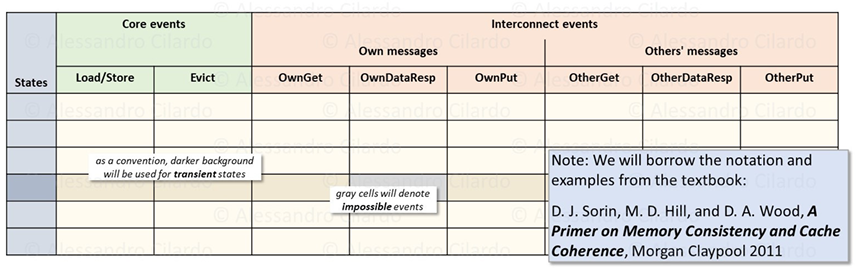
\includegraphics[width=0.8\textwidth]{fig/chapter_3/FSM.png}}
\end{figure}

\begin{info}
    Una macchina a stati finiti funziona descrivendo un sistema che può trovarsi in un insieme limitato di stati e che cambia stato in base agli ingressi ricevuti. In ogni istante la macchina si trova in uno stato ben preciso, detto stato corrente. Quando riceve un input, consulta le regole di transizione per capire in quale nuovo stato deve andare. A seconda del modello, la macchina può anche produrre un output che dipende solo dallo stato (nel caso di una FSM di Moore) oppure dallo stato e dall'input ricevuto (nel caso di una FSM di Mealy). Questo meccanismo rende le FSM particolarmente utili per descrivere sequenze di eventi o sistemi di controllo.
    Per rappresentarla in una tabella si usa una struttura che mette in relazione gli stati correnti con gli ingressi e specifica quale sarà lo stato successivo e, se previsto, l'output. Una riga della tabella corrisponde a una coppia formata dallo stato corrente e dall'input, mentre le colonne riportano lo stato verso cui si passa e l'eventuale valore di uscita. In questo modo, la tabella diventa una mappa compatta e leggibile che descrive completamente il comportamento della macchina.
\end{info}

\noindent
Un messaggio di tipo \textbf{Get} rappresenta una \textit{richiesta di lettura o allocazione} di un blocco di memoria. Esso viene tipicamente generato da un core quando si verifica un 
\textit{cache miss}, al fine di occupare una linea della cache con il blocco richiesto. 
L'informazione relativa al tipo di richiesta è codificata nel campo \textit{type} del messaggio. 
Quando un core osserva sull'interconnessione un messaggio di tipo Get emesso da un altro core, esso viene interpretato come \textbf{other Get}. In questo caso, il controller deve verificare se il blocco richiesto è eventualmente presente nella propria cache, per rispondere o per aggiornare lo stato del blocco secondo il protocollo di coerenza adottato.  

\noindent
Il messaggio di tipo \textbf{Put}, invece, è un'operazione di \textit{invio proattivo} di un blocco dalla cache verso il livello inferiore della gerarchia. Ciò avviene tipicamente in caso di \textit{eviction}, ossia quando una linea di cache deve essere liberata. In modo analogo al caso precedente, se un core osserva sull’interconnessione un messaggio di tipo Put proveniente da un altro core, questo viene classificato come \textbf{other Put}.  

\noindent
È importante notare che l'emissione di una richiesta da parte di un cache controller non implica necessariamente la sua immediata accettazione: l'interconnessione può infatti trovarsi in stato \textit{busy}. Per questo motivo, il controller mantiene visibilità delle proprie richieste sotto forma di \textbf{own messages}, che fungono da meccanismo di \textit{acknowledgment} da parte dell'interconnessione, consentendo di sincronizzare la generazione e l'elaborazione dei messaggi.  

\subsection{Protocollo a due stati con Writeback}
In questo protocollo basilare entrambe le FSM hanno due stati, V (Valid) e I (Invalid).
Per le FSM delle cache, V significa che il blocco è disponibile nella cache per lettura/scrittura, mentre I significa che il blocco non è presente in cache. Per l'FSM dell'LLC, V significa che il blocco è in qualche cache di livello superiore, I significa che è disponibile solo nell'LLC. 

\noindent Questo protocollo rispetta gli invarianti di coerenza, ma non supporta molteplici repliche dei dati in nodi diversi quando sono usati solo per operazioni di lettura. 

\begin{warn}
    Lavoriamo sotto l'ipotesi che tutti i messaggi sono inviati in broadcast a tutti i controller e sono visti da tutti nello stesso ordine. Un'ulteriore ipotesi è che gli eventi interni e di interconnesione sono \textit{simultanei} (Load miss $\rightarrow$ OwnGet + DataResp).
\end{warn}

\begin{figure}[ht]
    \centering
    \setlength{\fboxrule}{0.5pt} % spessore sottile
    \setlength{\fboxsep}{0pt}    % senza spazio interno
    \fbox{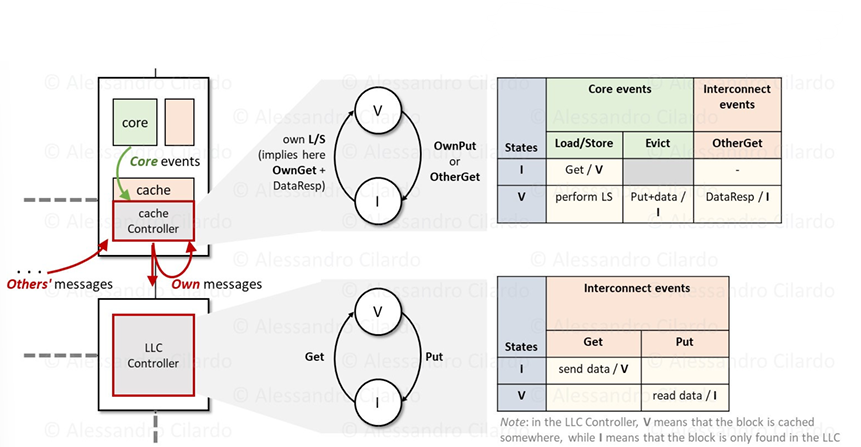
\includegraphics[width=0.85\textwidth]{fig/chapter_3/two_state_protocol.png}}
\end{figure}

\noindent Tipicamente l'interconnessione supporta messaggi di controllo e dato separati, perchè i dati hanno bisogno di risorse di interconnessione (bus) dedicati e impiegano molto più tempo rispetto alle informazioni di controllo. 
Di conseguenza, un interazione di richiesta/risposta deve necessariamente essere gestita da due messaggi separati: Il messaggio di richiesta risposta e il messaggio contenente i dati. \uppercase{è} necessario introdurre degli stati \textit{transienti}, per gestire la situazione in cui un messaggio di controllo è arrivato, ma non sono arrivati i dati. 

\begin{warn}
    Per ora assumiamo che se un core sta aspettando i dati in uno stato transiente, non può intervenire una get proveniente da un altro core. 
\end{warn}

\begin{figure}[ht]
    \centering
    \setlength{\fboxrule}{0.5pt} % spessore sottile
    \setlength{\fboxsep}{0pt}    % senza spazio interno
    \fbox{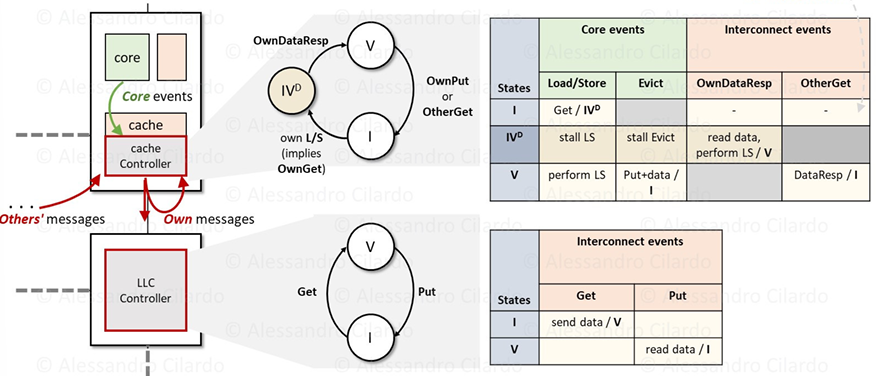
\includegraphics[width=0.85\textwidth]{fig/chapter_3/two_state_protocol_2.png}}
\end{figure}

\subsection{Protocollo a tre stati}
Per permettere la lettura simultanea di dati condivisi, mantenendo l'invariante SWMR, introduciamo il protocollo a tre stati \textbf{Modified-Shared-Invalid}. Questo protocllo permette di avere repliche dei dati in cache diverse, tranne per il caso in cui un core vuole scrivere il dato. Dal punto di vista dei core, è necessario distinguere richieste di blocchi che saranno solo letti e richiesti di blocchi che invece dovranno essere scritti. Questo implica la distinzione tra messaggi \textit{getS} (Get Shared) e \textit{getM} (Get Modified). Analogamente servirebbe una distinzione tra i messaggi putM e putS, ma putS in questo caso è superfluo in quanto per l'eviction di un blocco in sola lettura non è necessaria comunicazione (\textit{eviction silente}).

\begin{figure}[ht]
    \centering
    \setlength{\fboxrule}{0.5pt} % spessore sottile
    \setlength{\fboxsep}{0pt}    % senza spazio interno
    \fbox{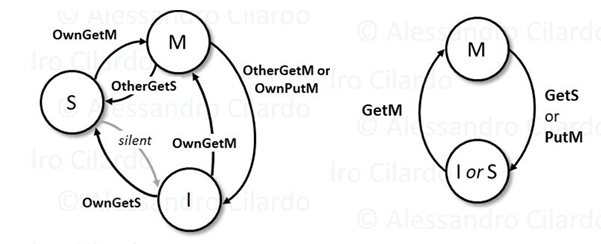
\includegraphics[width=0.6\textwidth]{fig/chapter_3/3_state_fsm.png}}
\end{figure}

\noindent Dal punto di vista dell'LLC, è interessante tracciare solo due stati: o una linea può essere modificata da qualche core oppure \textit{indifferentemente} o qualcuno può solo leggerla o ce l'ha solo LLC. 

\begin{figure}[ht]
    \centering
    \setlength{\fboxrule}{0.5pt} % spessore sottile
    \setlength{\fboxsep}{0pt}    % senza spazio interno
    \fbox{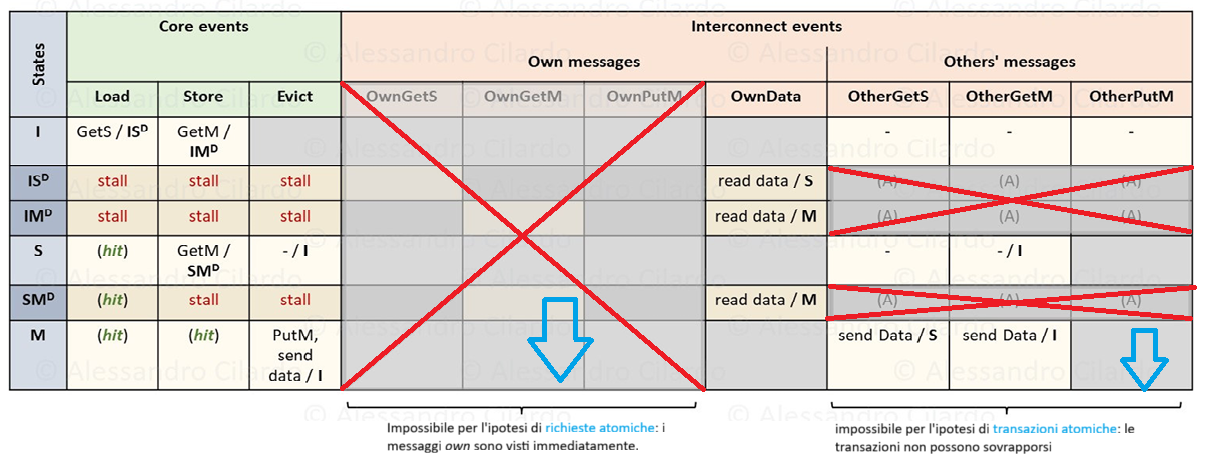
\includegraphics[width=0.95\textwidth]{fig/chapter_3/3_state_table.png}}
\end{figure}

\begin{figure}[ht]
    \centering
    \setlength{\fboxrule}{0.5pt} % spessore sottile
    \setlength{\fboxsep}{0pt}    % senza spazio interno
    \fbox{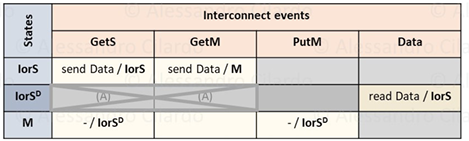
\includegraphics[width=0.55\textwidth]{fig/chapter_3/3_state_table_LLC.png}}
\end{figure}

\subsection{Lo stato Exclusive}
\uppercase{è} possibile espandere il numero di stati possibili per gestire al meglio determinate situazioni ricorrenti. Lo stato \textbf{Exclusive} serve a gestire i casi di Load $\rightarrow$ Store. Questp stato è usato in quasi tutti i protocolli di coerenza in commercio, in particolare nei processori ARM. Questo stato ottimizza il caso in cui un core inizialmente legge un blocco, e poi lo sovrascrive. Con il protocollo a tre stati questa situazione è descritta dalla sequenza load miss $\rightarrow$ GetS $\rightarrow$ Write Miss $\rightarrow$ GetM. Aggiungendo lo stato Exclusive, il controller può \textit{silenziosamente} aggiornare lo stato della linea da E $\rightarrow$ M, ma chiaramente solo se è l'unico core ad avere in cache attualmente la linea. 

\begin{warn}
    In realtà al posto di GetM andrebbe usato \textit{Update}, perchè è inutile trasportare i dati di nuovo dopo la GetS.
\end{warn}

\begin{figure}[ht]
    \centering
    \setlength{\fboxrule}{0.5pt} % spessore sottile
    \setlength{\fboxsep}{0pt}    % senza spazio interno
    \fbox{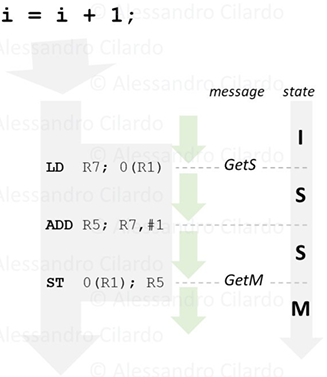
\includegraphics[width=0.35\textwidth]{fig/chapter_3/common_situation.png}}
\end{figure}

\noindent \uppercase{è} possibile implementare questo protocollo facendo in modo che il controller LLC abbia traccia di quante caches abbiamo il blocco nello stato S, attraverso un contatore e ricevendo i messaggi PutS, usati dalle cache quando vogliono fare un'operazione di \textit{evict} che fino a questo momento era rimasta silente. In questo modo il controller LLC può tenere traccia di quanti \textit{sharers} esistono, ma al contempo questo aumenta notevolmente il traffico di messaggi per la gestione della coerenza. 

\noindent Esiste una versione \textit{imperfetta} ma meno costosa, che consta di un approccio conservativo. Il controller LLC setta lo stato E di una linea su una prima richiesta di accesso, e nei successivi accessi lo stato muta E $\rightarrow$ S, e non torna mai più allo stato E, anche quando resta solo uno sharer.  

\begin{figure}[ht]
    \centering
    \setlength{\fboxrule}{0.5pt} % spessore sottile
    \setlength{\fboxsep}{0pt}    % senza spazio interno
    \fbox{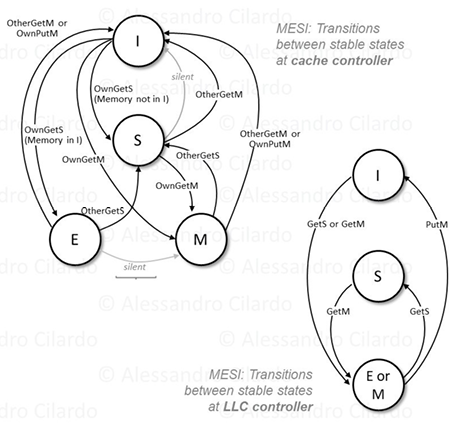
\includegraphics[width=0.55\textwidth]{fig/chapter_3/exclusive_fsm.png}}
\end{figure}

\subsection{Lo stato Owned}
\uppercase{è} possibile introdurre lo stato owner: un \textbf{Owner} è la cache che dispone della versione più aggiornata di una linea. Una cache in stato \textbf{O} deve rispondere alle richieste di altre cache per quel blocco, sollevando il controller LLC da questo onere. Quando una cache ha un blocco nello stato M oppure E, e riceve una GetS da un altro core, nel protocollo MSI, la cache deve rispondere mandando il dato al richiedente e al controller LLC, delegando la \textit{ownership} all'LLC. Il protocollo che include lo stato owned elimina il passaggio per l'LLC.


\subsection{Recap Stati di coerenza}
Dei protocolli visti finora possiamo sintetizzare i vari stati:

\begin{itemize}
    \item \textbf{Modified}: Il blocco è valido, exlusive, owned, e potenzialmente sporco;
    \item \textbf{Shared}: Il blocco è valido ma non esclusivo, pulito e non owned;
    \item \textbf{Invalid}: Il blocco è invalido:
    \item \textbf{Owned}: Il blocco è valido, owned, potenzialmente sporco ma non exclusive;
    \item \textbf{Exclusive}: Il blocco è valido, exclusive e pulito;
\end{itemize}

\begin{figure}[ht]
    \centering
    \setlength{\fboxrule}{0.5pt} % spessore sottile
    \setlength{\fboxsep}{0pt}    % senza spazio interno
    \fbox{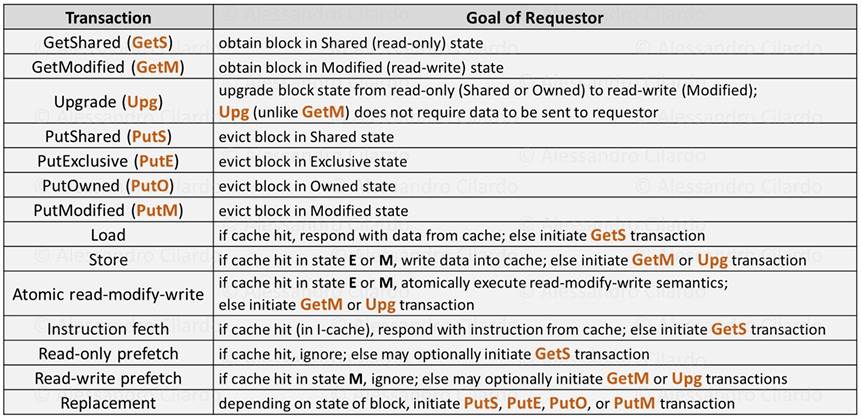
\includegraphics[width=0.9\textwidth]{fig/chapter_3/coherence_events.png}}
\end{figure}

\subsection{Rimozione delle ipotesi}
Nella trattazione fin qui presentata, sono state fatte delle potesi semplificative, che possono essere rimosse complicando il protocollo. Le ipotesi finora assunte sono:

\begin{itemize}
    \item \textbf{Richieste atomiche}: Ogni richiesta è accettata dall'interconnesione e notificata al sistema appena viene emessa dal core, non sussiste nessun intervallo di tempo tra l'evento interno e la comparsa del corrispondente messaggio sull'interconnessione;
    \item \textbf{Transazioni atomiche}: Le transazioni non possono sovrapporsi. Una volta che un messaggio di inizializzazione transazione viene accettato, nessun altro messaggio di transazione può essere accettato prima del trasferimento dei dati dati che completa la precedente transazione. La transazione non accettata risulta in uno stallo dell'evento nel core che l'ha generata;
    \item \textbf{Arbitraggio centralizzato}: Tutti i messaggi sono trasmessi in broadcast a tutti i controller e sono visti \textit{nello stesso ordine}. Questo ordine è garantito dell'interconnessione, che agisce da arbitro centralizzato e determina la consistente sequenza di eventi vista da tutti i controllori. 
\end{itemize}

\noindent La rimozione di queste ipotesi introduce protocolli più sofisticati che contemplano più stati transienti. Iniziamo rimuovendo l'ipotesi di \textbf{Richieste atomiche}. È necessario adesso considerare una coda di messaggi tra il controller della cache e il bus, in modo che ci sia un delay temporale tra il momento in cui una richiesta è emessa dal controller e il momento in cui viene \textit{ordinata}. Questo comporta un gran numero di stati transienti aggiuntivi. 
Ad esempio, è necessario introdurre un nuovo stato che contempli l'attesa dell'ACK per una richiesta emessa da parte dell'interconnesione, secondo la trafila $\text{I} \rightarrow \text{IS}^{AD} \rightarrow \text{IS}^{D} \rightarrow S$. Il passaggio tra il penultimo stato e l'ultimo stato è semplice in quanto stiamo ancora facendo l'ipotesi di transazioni atomiche. 

\begin{figure}[ht]
    \centering
    \setlength{\fboxrule}{0.5pt} % spessore sottile
    \setlength{\fboxsep}{0pt}    % senza spazio interno
    \fbox{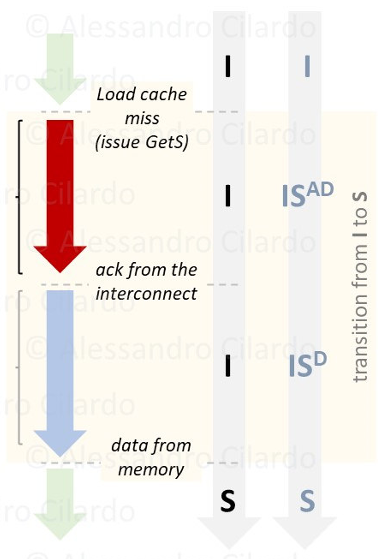
\includegraphics[width=0.3\textwidth]{fig/chapter_3/esempio_rimozione_ipotesi.png}}
\end{figure}

\noindent \uppercase{è} interessante osservare che nella notazione introdotta per gli stati, per gli stati transienti il primo stato a comparire della coppia è lo stato in cui \textit{effettivamente} il blocco risulta ancora essere nonostante la transizione, e il sistema si comporta di conseguenza. Rimuoviamo ora l'ipotesi di \textbf{arbitraggio centralizzato}. 

\begin{info}
    Lo snooping è una tecnica in cui tutte le cache collegate a un bus condiviso monitorano costantemente le transazioni che vi transitano, con lo scopo di mantenere la coerenza dei dati. Ogni volta che un processore esegue un'operazione di lettura o scrittura in memoria, tale operazione viene propagata sul bus e tutte le cache osservano (snoop) l'evento per verificare se possiedono una copia della linea di cache coinvolta. In base allo stato della linea di cache, determinato dal protocollo adottato, ciascuna cache può invalidare la propria copia se un altro processore ha scritto su quella linea, fornire i dati direttamente al richiedente se possiede la copia aggiornata, oppure aggiornare la linea secondo le regole del protocollo. In questo modo, lo snooping assicura che tutte le copie di una stessa cella di memoria distribuite nelle diverse cache rimangano consistenti, evitando che un processore lavori su dati obsoleti.
\end{info}

\noindent Nei protocolli basati sullo snooping tutte le richieste da parte di un controller vengono trasmesse in broadcast a tutti gli altri controllori, incluso se stesso. Ipotesi fondamentale per questa modalità è che la rete di interconnesisone garantisca un ordinamento completo. Il bus condivisio agisce da \textit{ordinatore}, in particolare per le operazioni di scrittura. Lo scopo è mantenere l'invariante SWMR. I vincoli dell'ordine si applicano soprattutto alle richieste, poichè è necessario che sia ordinata la richiesta trasmessa in broadcast, mentre la risposta unicast arriva dopo solo al richiedente. I messaggi DATA possono viaggiare su una rete separata. Nonostante ciò, i protocolli basati su \textit{snooping} non scalano bene . Infatti su una macchina composta da N nodi, ci saranno almeno N interazioni per ogni cache miss, e questo implica un traffico non sostenibile a livello di latenza sul bus che agisce da collo di bottiglia per sistemi con molti nodi. 

\subsection{Directory}
Soluzione alternativa ai protoclli basti sullo snooping maggiromente scalabile. La \textbf{Directory} è di fatto un componente del sistema che tiene traccia globalmente dello stato di coerenza di tutti i blocchi. Questo registro viene consultato per scoprire informazioni su un blocco nelle altre caches, dove si trova anche la corrente locazione delle copie. Il grande vantaggio di questa soluzione è che queste informazioni sono scambiante in modalità unicast ovvero point2point. La diretory inoltre è logicamente unificata, ma in pratica può essere distribuita su più nodi per aumentare la scalabilità.  


\begin{figure}[ht]
    \centering
    \setlength{\fboxrule}{0.5pt} % spessore sottile
    \setlength{\fboxsep}{0pt}    % senza spazio interno
    \fbox{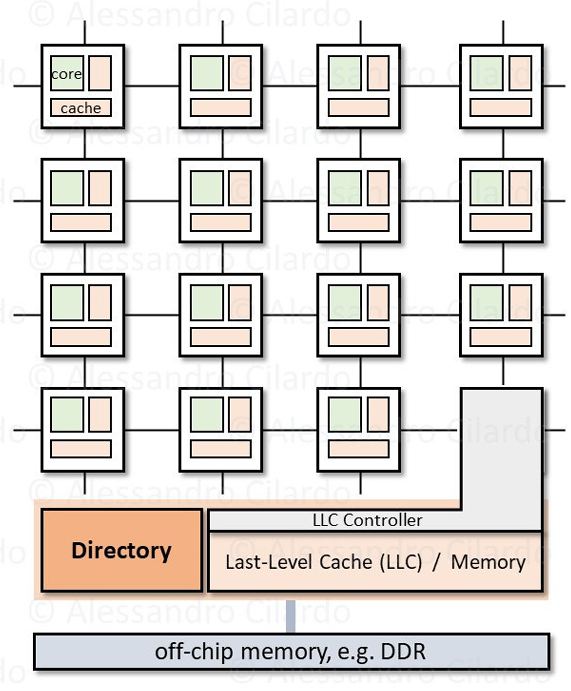
\includegraphics[width=0.5\textwidth]{fig/chapter_3/directory.png}}
\end{figure}


\noindent Di base il protocollo basato di directory prevede che le singola caches mandini tutte le richieste ad una singola directory, che risponde alla richiesta o \textit{inoltra} il messaggio ad altri controllers per poi rispondere. Inoltre, la directory e talvolta i controller richiedenti, devono conoscere il numero di \textit{sharer} che condividono un blocco. 

\begin{warn}
    Il protocollo basato su directoy non specifica i dettagli implementativi della rete di interconnesione. Non deve necessarimente essere un bus condiviso, e richieste e risposte possono fluire in diversi canali.
\end{warn}

Per ogni blocco possiamo definire dei ruoli per i nodi:
\begin{itemize}
    \item \textbf{Home}: Nodo la cui memoria principale contiene la linea;
    \item \textbf{Dirty}: Nodo che in cache una copia del blocco ma sporca;
    \item \textbf{Owner}: Nodo che al momento mantiene la copia più recente del blocco e deve rispondere alle richieste per quel blocco;
    \item \textbf{Exclusive}: Unico nodo che ha il blocco, sia pulito che sporco;
    \item \textbf{Local}: Nodo che effettua una richiesta per il blocco. 
\end{itemize}

Assumiamo come ipotesi che l'interconnessione garantisca l'ordinamento point2point, ovvero che se un controller A manda due messaggi al controller B, allora i messaggi arrivano a B nello stesso ordine in cui sono partiti da A. 
Sotto quest'ipotesi la directory agisce la \textit{punto di serializzazione}, ovvero di ordinamento delle richiesta, ma, a differenza del protocollo basato su snooping, sono necessari messaggi di ack dagli sharers in quanto non c'è cognizione di un ordinamento totale o di serializzazione globale. Ipotizziamo inoltr LLC monolitici con un singolo \textit{Directory Controller}. 

\begin{figure}[ht]
    \centering
    \setlength{\fboxrule}{0.5pt} % spessore sottile
    \setlength{\fboxsep}{0pt}    % senza spazio interno
    \fbox{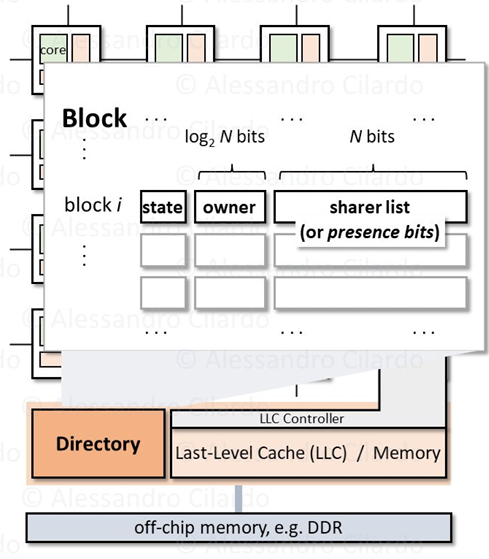
\includegraphics[width=0.5\textwidth]{fig/chapter_3/directory_2.png}}
\end{figure}

Assumiamo che il sistema consti di N nodi (cores). Il registro contenuto inDirectory tiene traccia di quale cache ospita quale blocco e in che stato, e mantiene lo stato ogni blocco. Per ogni blocco, usa un vettore di N bit denominato \textbf{presence bits}, insieme ai bit per indicare lo stato. Le informazioni conservate nella directory includono lo stato \textbf{stabile} di coerenza (I,O,M,...), l'identità dell'owner su $log_2N$ bits. Le informazioni della directory sono utilizzate e aggiornate in base al particolare protocollo di coerenza. 

\subsection{Protocollo Directory MSI}
Quando un core ha bisogno di una linea, la richiede alla Directory. Se lo stato della linea è \textbf{I} in Directory (ovvero presente in nessuna cache), allora i dati sono copiati dalla directory al richiedente, e analogamente accade se lo stato è \textbf{S}, indipendentemente da quanti sono gli sharer. Se il blocco è \textbf{O}, ovvero owned da un altro core e potenzialmente sporco, la Directory richiama il blocco dal proprietario, e ritrasmette i dati al richiedente (si può implementare un meccanismo per trasmettere i dati in parallelo al richiedente e alla Directory), e viene aggiornato lo stato: Il nuovo stato è \textbf{S} se arriva una GetS, è \textbf{M} se arriva una GetM, e in quest'ultimo caso aggiornare il campo owner con il nuovo proprietario. Prima di completare la transizione a M, la Directory contatta tutte le cache del presence bits individualmente e deve aspettare un ACK da tutte.

\noindent Questo protocollo può essere ottimizzato nel seguente modo:
\begin{itemize}
    \item Dato che non è necessario ordinare le risposte e non è necessario trasferirle in broadcast, queste possono viaggiare su una rete separata che non supporta broadcast e ordinamento;
    \item Eliminare l'ipotesi di Directory associata ad un singolo LLC: Più Directory indipendenti possono gestire la coerenza di diversi insiemi di blocchi. La Directory per un dato blocco è fissa in un solo posto, ma diversi blocchi possono avere diverse Directories. Ogni blocco ha una \textit{home}, ovvero una directory che ospita i dati e lo stato di directory;
    \item Riduzione dell'informazione conservata in Directory: Una entry nella sharer list corrisponde ad un gruppo di K caches, e se una o più caches di quel gruppo hanno il blocco potenzialmente è in stato S, allora viene alzato il bit. Questo però è inefficiente in quanto molti dei messaggi di \textit{invalidation}, che comunque devono essere mandati dalle cache, risultano inutili ai fini del mantenimento della bitmap. La soluzione consiste nel tenere traccia degli M blocchi (M<N) che hanno 0 o pochi sharer, in modo tale da ridurre i bit a $M\cdot log_2N$. Questo potrebbe però richiedere un meccanismo aggiuntivo per gestire il caso, comunque raro, di voler aggiungere un (M+1)esimo sharer.  
\end{itemize}

\begin{warn}
    I protocolli di coerenza possono introdurre deadlocks! Infatti la ricezione di un messaggio può scatenare l'invio di un messaggio di tipo \textit{forward}, e questi messaggi possono usare una risorsa comune (linee di rete, buffers o code). Una soluzione è l'uso di \textit{virtual networks}, che separano i messagi in classi, e vengono utilizzati buffer dedicati per ogni tipologia di messaggio, in modo da evitare cicli nel grafo delle dipendenze a livello di \textit{risorsa di rete}.
\end{warn}



